\documentclass[10pt]{article}
\usepackage{preference}

\usepackage{mdframed}
\usepackage{stmaryrd}
\mdfsetup{skipabove=1em,skipbelow=0em}
\theoremstyle{definition}
\newmdtheoremenv[nobreak=true]{statement}{Утверждение}
\newtheorem*{note}{Замечание}
\newcommand\true{\text{\textit{И}}}
\newcommand\false{\text{\textit{Л}}}

%опа, нашёл как жить

%бтв, Костя, можешь вставить вот это в преамбулу того, где нужно писать код (скорее всего только алгосы)

\usepackage{listings}

\definecolor{codegreen}{rgb}{0,0.6,0}
\definecolor{codegray}{rgb}{0.5,0.5,0.5}
\definecolor{codepurple}{rgb}{0.58,0,0.82}
\definecolor{backcolour}{rgb}{0.95,0.95,0.92}

\lstdefinestyle{myStyle}{
    backgroundcolor=\color{backcolour},   
    commentstyle=\color{codegreen},
    keywordstyle=\color{magenta},
    numberstyle=\tiny\color{codegray},
    stringstyle=\color{codepurple},
    basicstyle=\ttfamily\footnotesize,
    breakatwhitespace=false,         
    breaklines=true,                 
    captionpos=b,                    
    keepspaces=true,                 
    numbers=left,                    
    numbersep=5pt,                  
    showspaces=false,                
    showstringspaces=false,
    showtabs=false,                  
    tabsize=2,
    extendedchars=\true
}

\lstset{style=myStyle}

\lstset{language=Python}
\begin{document}

\def\chap#1#2{\ \\ {\large\bf#1 \ | \ \tt\scshape#2} \par}

\ \vspace{-1cm}

{\bf
\ \\
\Large\centerline{\scshape Матлог, лекции}
}\normalsize

% \section{Введение}

Логика -- довольно старая наука, но наш предмет довольно молодой
В какой-то момент логики как дисциплиниы, которая учит просто правильно рассуждать, стало нехватать.
Появилась теория множеств.
Общего здравого смысла не хватает, нужен строгий математичесий язык. 
Это рубеж 19-20 веков.

У нас теория множеств не будет фокусом, как это могло бы быть на мат. факультете.

Теория множеств, когда она была впервые сформулирована, была противоречива (как матан, сформулированный Ньютоном).
Чтобы уверенно и эффективно заниматься матаном, нужно суметь его формализовать. 

<Парадокс Рассела / парадокс брадобрея>
Мы приписываем элементу-человеку свойство, которое невыполнимо.
Обьекта, выходит, не существует.
Мы смогли очень быстро определить противоречие в этом определении.
Но, может быть, мы не смогли его определить в других наших определениях? 
(конструкциях вещественной прямой, и т.д и т.д)

Программа Гильберта.
\begin{enumerate}
\item Формализуем математику!
Сформулируем теорию на языке (не на русском или английском), который не будет допускать парадоксов, 
\item $\ldots$ и на котором можно будует доказать непротиворечивость. 
\end{enumerate}

В 1930 году становится понятно, что сколько-нибудь сильная (= в ней можно построить формальную арифметику) теория не может быть доказана непротиворечивой.

Возможно, сама наша логика неправильная? 
Эта идея будет нам полезна, и к ней мы ещё вернемся.

Возможно, что это просто свойство мира, и мы хотим невозможного.

Из этих рассуждений выросло большое множество хороших идей, которые оказались полезны в других местах.
Матлогика служит широкому кругу нужд.

Мы можем доказывать, что программа работае корректно. 
Именно доказывать, а не проверять тестами!

Мы можем изучать свойства самих языков.
Изоморфизм Карри-Говарда--- доказательство это программа, утверждения это тип.
Можно изучать языки программирования и можно развернуть изоморфизм: изучать математкиу как язык программирования. 

Функциональные языки: окамль + хаскель. 
Ознакомление с этими языками преставляет собой способ ознакомиться с предметом немного с другой стороны.

\section{Исчисление высказываний}
Мы говоирм на двух языках: на предметном языке и метаязыке.
Предметный язык -- это то, что изучается, а метаязык -- это язык, НА котором это изучается.

На уроках английского предметным является сам английский, а метаязыком может быть русский.
Метаязык -- это язык исследователя, а предметный язык -- это язык исследоваемого.
Что такое язык вообще? Хороший вопрос.

Высказывание --- это одно из двух: 
\begin{enumerate}
\item Большая латниская буква начала алфавита, возможно с индексами и штрихами --- это пропозициональные переменные.
\item Выражение вида $(\alpha \land \beta)$, $(\alpha \lor \beta)$, $(\alpha \to \beta)$, $(\neg \alpha)$. 
\end{enumerate}

В определении выше альфа и бета это метапеременные--- места, куда можно подставить высказывание.
\begin{enumerate}
\item $\alpha, \beta, \gamma$ --- метапеременные для всех высказываний.
\item $X, Y, Z$ --- метапеременные для пропозициональных переменных.
\end{enumerate}

Метапеременные являются частью языка исследователя.

В формализации мы останавливаемся до места, в котором мы можем быть уверены, что сможем написать программу, которая всё проверяет.

Сокращение записи, приоритет операций: сначала $\neg$, потом $\&$, потом $\vee$, потом $\to$.
Если скобки опущены, мы восстанавливаем их по приоритетам.
Выражение без скобок является частью метаязыка, и становится частью предметного, когда мы восстанавливаем их.
Скобки последовательных импликаций расставляются по правилу правой ассоциативности --- справа налево.
\subsection{Теория моделей}
У нас есть истинные значения $\{T, F\}$ в классической логике. 
И есть оценка высказываний $\llbracket \alpha\rrbracket$. 
Например $\llbracket A \lor \neg A\rrbracket$ истинно.
Всё, что касается истинности высказываний, касается теории моделей. 
\begin{definition}
    Оценка --- это функция, сопоставляющая высказыванию его истинное (истинностное) значение.
\end{definition}
\subsection{Теория доказательств}
\begin{definition}
    Аксиомы --- это список высказываний.
    Схема аксиомы --- высказывание вместе с метопеременными; при любой подстановке высказываний вместо метапеременной получим аксиому. 
\end{definition}

\begin{definition}
    Доказательство (вывод) --- последовательность высказываний $\gamma_1, \gamma_2\ldots$ где $\gamma_i$--- любая аксиома, 
    либо существуют $j,k < i$ такие что $\gamma_j \equiv (\gamma_k \to \gamma_i)$.
    (знак $\equiv$ здесь сокращение для "имеет вид"). Это правило ''перехода по следствию'' или Modus ponens.
\end{definition}

Определим следующие 10 схем аксиом для того исчисления высказываний, которое мы рассматриваем. 
\begin{enumerate}
    \item $\alpha \to \beta \to \alpha$~--- добавляет импликацию
    \item $(\alpha \to \beta) \to (\alpha \to \beta \to \gamma) \to (\alpha \to \gamma)$~--- удаляет импликацию
    \item $\alpha \land \beta \to \alpha$~--- удаление конъюнкции
    \item $\alpha \land \beta \to \beta$~--- удаление конъюнкции
    \item $\alpha \to \beta \to \alpha \land \beta$~--- внесение конъюнкции
    \item $\alpha \to \alpha \lor \beta$~--- внесение дизъюнкции
    \item $\beta \to \alpha \lor \beta$~--- внесение дизъюнкции
    \item $(\alpha \to \gamma) \to (\beta \to \gamma) \to (\alpha \lor \beta \to \gamma)$
    \item $(\alpha \to \beta) \to (\alpha \to \neg \beta) \to (\neg \alpha)$
    \item $\neg \neg \alpha \to \alpha$ --- очень спорная штука.
\end{enumerate}

\begin{example} Доказательство
    $\vdash A \to A $.
    \begin{enumerate}
        \item $A \to (A \to A) \to A$ (схема 1)
        \item $A \to A \to A$  (схема 1)
        \item $(\underbrace{A}_\alpha \to \underbrace{A \to A}_\beta) \to (\underbrace{A}_\alpha \to \underbrace{(A \to A)}_\beta \to \underbrace{A}_\gamma) \to (\underbrace{A}_\alpha \to \underbrace{A}_\gamma)$  (схема 2)
        \item $(A \to (A \to A) \to A) \to (A \to A)$ (m.p 2, 3)
        \item $A \to A$ (m.p 1, 4)
    \end{enumerate}
\end{example}
% \subsection{Теорема о дедукции}

\begin{definition}
    (Метаметаопределение).
    Будем большими греческими буквами $\Gamma, \Delta, \Sigma\ldots$ --- списки формул, неупорядоченные.
\end{definition}

\begin{definition}
    Вывод из гипотез: $\Gamma \vdash \alpha$.

    То есть существует $\delta_1,\dots, \delta_n$,~$\delta_n \equiv \alpha$, где $\delta_i$ или аксиома, гипотеза или m.p. из $j$ и $k$ и $j, k < i$.
\end{definition}

\begin{theorem}
    $ \Gamma, \alpha \vdash \beta$ тогда и только тогда, когда $\Gamma \vdash \alpha \to \beta$.
\end{theorem}

\begin{proof}
    \begin{itemize}
        \item [$\Leftarrow $]
        Пусть $\delta_1, \delta_2\ldots \delta_n \equiv \alpha \to \beta$ выводит $\alpha \to \beta$.
        Дополним этот вывод до доказательства двумя новыми высказываниями: $\delta_{n+1} \equiv \alpha$ (дано нам в гипотезе), $\gamma_{n+2} \equiv \beta$ (MP шагов $n$, $n+1$) --- это и требовалось.
        \item [$\Rightarrow $]  Пусть $\Gamma, \alpha \vdash \beta$. Напишем программу, которая построит $\Gamma \vdash \alpha \to \beta$.

        Инвариант, который мы будем поддерживать: всё до $\alpha \to \delta_i $ --- док-во.
        Доказательство индукцией по $n$.
        \begin{enumerate}
            \item База: $n=1$ --- без комментариев.
            \item Если $\delta_1,\ldots, \gamma_n$ можно перестроить в доказательство $\alpha \to \gamma_n$, то $\gamma_1 \ldots \gamma_{n+1}$ тоже можно перестроить.
            Разберём случаи:
            \begin{enumerate}
                \item $\delta_i$ --- аксиома или гипотеза из $\Gamma$. \\
                ($i - 0.6$) $\delta_{i}$ \\
                ($i - 0.3$) $\delta_i \to \alpha \to \delta_i$\\
                ($i$) $\alpha \to \delta_i$ (m.p из $i-0.6$ и $i - 0.3$)
                \item $\delta_i = \alpha$, то есть надо построить $\alpha \to \alpha$\\
                ($i - 0.8, i-0.6, i-0.4, i-0.2$) (доказательство $\alpha \to \alpha$) \\
                $(i)$ $\alpha\to\alpha$
                \item $\delta_i$ получено из $\delta_j$ и $\delta_k$ ($\delta_k \equiv \delta_j \to \delta_i$)\\
                по индукционному предположению, уже есть строчки вида $\alpha \to \delta_j, \alpha \to \delta_k$\\
                ($j$) $\alpha \to \delta_j$\\
                ($k$) $\alpha \to (\delta_j \to \delta_i)$\\
                ($i - 0.6$) $(\alpha \to \delta_j) \to (\alpha \to \delta_j \to \delta_i) \to (\alpha \to \delta_i)$ (схема 2)\\
                ($i - 0.3$) $(\alpha \to \delta_j \to \delta_i) \to (\alpha \to \delta_i)$ (m.p.)\\
                ($i$) $(\alpha \to \delta_i)$ (m.p.)
            \end{enumerate}
        \end{enumerate}
    \end{itemize}
\end{proof}

\subsection{Теория моделей}
Мы можем доказывать модели или оценивать их.
<<Мы можем доказать, что мост не развалится или можем выйти и попрыгать на нём.>>

\begin{definition}
    $\mathbb{V}$~--- истинностное множество.

    $F$~--- множество высказываний нашего исчисления высказываний.

    $P$~--- множество пропозициональных переменных.
    \[ \llbracket\cdot\rrbracket: F \to \mathbb{V} \text{~--- оценка}\]
\end{definition}

\begin{definition}
    Для задания оценки необходимо задать оценку пропозициональных переменных.
    \[\llbracket \cdot \rrbracket : P\to \mathbb{V} \quad f_P\]
    Тогда:
    \[ \llbracket x \rrbracket = f_p(x)\]
\end{definition}

\begin{remark}
    Обозначение: значения пропозициональных переменных будем определять в верхнем индексе: $\llbracket \alpha \rrbracket ^{A = \true, B = \false \ldots}$.
\end{remark}


\begin{definition}
    $\alpha$ --- общезначимая (истинна), если $\llbracket \alpha \rrbracket = \true$ при любой оценке $P$.

    $\alpha$ --- невыполнима (ложна), если $\llbracket \alpha \rrbracket = \false$ при любой оценке $P$.

    $\alpha$ --- выполнима, если $\llbracket \alpha \rrbracket = \true$ при некоторой $f_P$.

    $\alpha$ --- опровержима, если $\llbracket \alpha \rrbracket = \false$ при некоторой $f_P$.
\end{definition}

\begin{definition}
    Теория корректна, если доказуемость влечёт общезначимость.

    Теория полна, если общезначимость влечёт доказуемость.
\end{definition}

\begin{definition}
    $\Gamma \vDash \alpha$ означает, что $\alpha$ следует из $\Gamma = \{ \gamma_1, \ldots, \gamma_n\}$, если $\llbracket \alpha \rrbracket = \true$ всегда при $\llbracket \gamma_i \rrbracket = \true$ при всех $i$.
\end{definition}

\subsection{Корректность исчисления высказываний}
\begin{theorem}
    Исчисление высказываний корректно.
    $\vdash \alpha$ влечёт $\vDash \alpha$.
\end{theorem}
\begin{proof}
    Индукция по длине доказательства $\delta_1, \dots, \delta_n$.

    Разбор случаев:
    \begin{enumerate}
        \item $\delta_i$ аксиома $\implies$ построить таблицу истинности, проверить, что все верно.
        \item $\delta_i$ --- м.п. $\delta_j$, $\delta_k \equiv \delta_j \to \delta_i \implies$ также рассмотрим таблицу истинности.
    \end{enumerate}
\end{proof}

Мы даём доказательство на метаязыке, не пускаясь в отчаянный формализм.
Такая строгость нас устраивает.

В матлогике бессмысленно формализовывать русский язык.
Она нужна, чтобы дать ответы на сложные вопросы в математике, где здравого смысла недостаточно и нужна формализация.

\subsection{Полнота исчисления высказываний}
\begin{theorem}
    Исчисление высказываний полно.
\end{theorem}

\begin{definition}
    $_{[\beta]}\alpha =
    \begin{cases}
        \alpha, & \llbracket \beta \rrbracket = \true\\
        \neg \alpha,&  \llbracket \beta \rrbracket = \false\\
    \end{cases}$
\end{definition}

\begin{lemma}
    $_{[\alpha]}\alpha$, $_{[\beta]}\beta \vdash _{[\alpha \star \beta]} \alpha \star \beta$, \\
    $_{[\alpha]} \alpha \vdash _{[\neg \alpha]}\neg\alpha $
\end{lemma}
\begin{proof}
    [Доказательство было в дз]
\end{proof}
\begin{example}
    $\llbracket \alpha \rrbracket = \true, \llbracket \beta \rrbracket = \false \implies  \alpha \wedge \neg \beta \vdash \neg (\alpha \wedge \beta) $.
\end{example}

\begin{lemma}
Если $\Gamma \vdash \alpha$, то $\Gamma, \Delta \vdash \alpha$.
\end{lemma}

\begin{lemma}
Пусть дана $\alpha$, $X_1,\ldots, X_n$ --- её переменные.

\[ _{[X_1]}X_1,\ldots _{[X_n]}X_n\ \vdash _{[\alpha]}\alpha  \]
\end{lemma}
\begin{proof}
    Пусть $\tl X = _{[X_1]} X_i \dots _{[X_n]} X_n$.

    Индукция по длине формулы $\alpha$.\\
    База: $\alpha = X_i$.\\
    Переход: есть $\alpha, \beta$. По предположению $\tl X \vdash _{[\alpha]} \alpha ~~~ \tl X \vdash _{[\beta]} \beta$.

    По лемме 1 тогда  $\tl X \vdash _{[\alpha \star \beta]} \alpha \star \beta$.
\end{proof}

\begin{lemma}
    Если $\vDash \alpha$, то при любой оценке $\tl X \vdash \alpha$.
    То есть при любых подстановках значений $\alpha $ будет истинна.
\end{lemma}

\begin{lemma}
    \[ \Gamma, Y \vdash \alpha, \quad \Gamma, \neg Y \vdash, \text{ то } \Gamma \vdash \alpha \]
\end{lemma}
\begin{proof}[Доказательство было в дз]
\end{proof}

\begin{lemma}
    Если $\tl X \vdash \alpha$ при всех оценках $X_1, \dots, X_n$, то $\vdash \alpha$.
\end{lemma}
\begin{proof}
    [Доказательство индукцией по $n$]
\end{proof}
\addtocounter{theorem}{-1}
\begin{theorem}
    Исчисление высказываний полно. Если $\vDash \alpha$, то $\vdash \alpha$.
\end{theorem}
\begin{proof}
    По лемме 4 и лемме 6.
\end{proof}

\section{Интуиционистская логика}
Мы не хотим дурацких конструкций вроде парадокса брадобрея.
Мы не хотим странных, но логически верных утверждений вроде $A\to B \lor B \to A$.
Интуиционистская логика предлагает свою математику, в которой своя интерпретация логических связок.
ВНК-интерпретация (Брауер-Гейтинг-Колмогоров).

\begin{itemize}\itemsep=-1mm
    \item $\alpha, \beta, \gamma \ldots$ --- это конструкции.
    \item $\alpha \land \beta$ если мы умеем строить и $\alpha$, и $\beta$.
    \item $\alpha \lor \beta$, если мы умеем строить $\alpha, \beta$ и знаем, что именно.
    \item $\alpha \to \beta$, если мы умеем перестроить $\alpha$ в $\beta$.
    \item $\bot $ --- не имеет построения
    \item $\neg \alpha \equiv \alpha \to \bot$
\end{itemize}

''Теория доказательств''.
Рассмотрим классическое исчисление высказываний и заменим схему аксиом 10 на следующую
\[ \alpha \to \neg \alpha \to \beta \]

В этой формализации мы следуем не сути интуиционистской логики, а традиции.
В интуиционистской логике формализм это не источник логики.

Примеры моделей.
\begin{enumerate}
    \item Модели КИВ подходят: корректны, но не полны ($\llbracket A \lor \neg A \rrbracket = \true$, но $\not\vdash_{\text{И}} A \lor \neg A$).
    \item Пусть $X$ топологическое пространство.

    Пусть истинностные значения~--- все открытые пространства в классической топологии.
    \begin{itemize}
        \item $\llbracket \alpha \& \beta \rrbracket = \llbracket \alpha \rrbracket \cap \llbracket \beta \rrbracket$.
        \item $\llbracket \alpha \lor \beta \rrbracket = \llbracket \alpha \rrbracket \cup \llbracket \beta \rrbracket$.
        \item $\llbracket \alpha \to \beta \rrbracket = \left( X \setminus \llbracket \alpha \rrbracket \cup \llbracket \beta \rrbracket \right)^{o}$.
        \item $\llbracket \neg \alpha\rrbracket = \left(X \setminus \llbracket \alpha \rrbracket \right)^{o}$.
    \end{itemize}
\end{enumerate}
\begin{theorem}
    Топологические модели~--- корректные модели ИИВ.
\end{theorem}
\begin{statement}
    $\not\vdash_{\text{И}} A \lor \neg A $.
\end{statement}
\begin{proof}
    Пусть $A = (0, +\infty)$, $\neg A = (-\infty, 0)$, $A \lor \neg A = \R \setminus \{0\} \neq \R$.
\end{proof}

\endinput

% \section{Общая топология}

Раньше были телевизоры с \textit{бесконченым} количеством пикселей (это зависит от химических свойств вещества кинескоп).

\begin{center}
    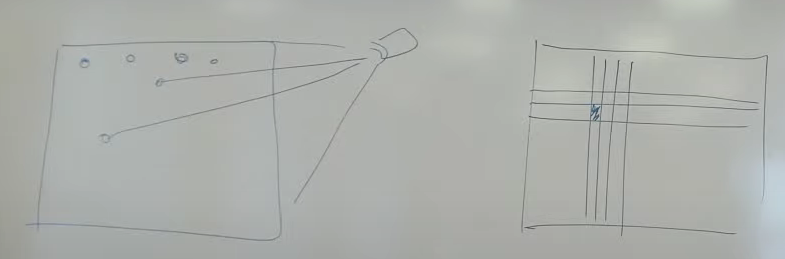
\includegraphics[scale=0.8]{parts/topology_tv_example}
\end{center}

Возьмем множество $X$. Определим на нем топологию как подмножество множества всех подмножеств
$\Omega \subseteq \mathcal{P}(X)$. $\Omega$ --- топология, если это множество открытых множеств и выполнены следующие условия:
\begin{enumerate}
    \item $\varnothing, X \in \Omega$;
    \item $\bigcup\limits_i \in \Omega$, если все $A_i \in \Omega$;
    \item $\bigcap\limits_{i = 1} ^ n A_i \in \Omega$, если $A_1, \dots, A_n \in \Omega$.
\end{enumerate}

То есть топологическое пространство~--- пара $\langle X, \Omega \rangle$ и про $\Omega$ верны приведенные выше три утверждения.

\begin{definition}
[Замкнутое мноежство] Множество $B$ такое, что $X \setminus B \in \Omega$ называется замкнутым.
\end{definition}

\begin{definition}
    [Связное топологическое пространство] $\langle X, \Omega \rangle$ связно, если нет $A, B \in \Omega ~:~ A \cup B = X$ и $A \cap B = \varnothing$
\end{definition}
    
\begin{definition}[Подпространство]
    $\langle X_1, \Omega_1 \rangle $ --- подпространство $\langle X, \Omega \rangle$, если
    $X_1 \subseteq X$ и $\Omega_1 = \{ a \cap X_1 ~|~ a \in \Omega$ \}  
\end{definition}

\begin{definition}
    [Связное множество]

    Множество, являющееся связным подпространством.
\end{definition}

\begin{center}
    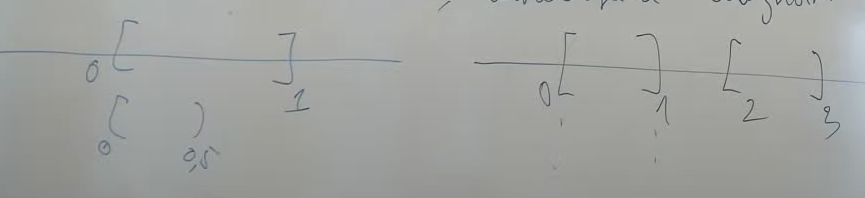
\includegraphics[scale=0.6]{parts/topology_connectivy}
\end{center}

\subsection{Примеры топологических пространств}
Возьмем дерево (граф). Множество $X$~--- множество вержин. $\Omega$~--- множество всех вершин, что
$B \in \Omega$, \underline{если} $a \in B$, $x \leqslant a$ влечет $x \in B$. 
То есть $\Omega$ --- семейство множеств вершин, которые входят вместе с поддеревом.  

\begin{theorem}
    Граф без цикла свяен тогда и только тогда, когда оно своязно как топологическое пространство.
    \begin{proof}[Доказательство будет в дз]
    \end{proof}
\end{theorem}

\begin{definition}[Решетки]
    $X$~--- частично упорядоченное множество отношением $\leqslant$.\\
    Множество верхних граней $a, b$ --- множество $\{ x \in X ~|~ a \leqslant x, b \leqslant x\}$.\\
    Множество нижних граней $a, b$ --- $a \sqcup b$ --- множество $\{ x \in X ~|~ a \geqslant x, b \geqslant x\}$.\\
    $A$, наименьший элемент $A$ --- такой $a \in A$, что нет $b \in A$, $b \leqslant a$.\\
    $a+b$ = наименьший элемент множества верхних граний.\\
    $a*b$ = наибольший элемент множества нижних граний.

    Решетка --- частично упорядоченное множество, где для каждых двух элементов существуют $a+b$ и $a*b$.
\end{definition}

\begin{example}
    Дерево --- не решетка (в общем случае), так как $a + b$ есть, а $a*b$ может не быть.
\end{example}

\begin{theorem}
    Пусть $\langle X, \Omega \rangle$ топологическое пространство, $A, B \in \Omega$. $A \leqslant B$, если $A \subseteq B$.

    Тогда $\langle \Omega, \leqslant\rangle$ --- решетка. $A \cdot B = A \cap B, ~ A + B = A \cup B$.
\end{theorem}

\begin{definition}
    Дистрибутивная решетка --- это такая решетка, что $a,b,c \in \Omega$, ~$a + (b \cdot c) = (a + b) \cdot (a + c)$.
\end{definition}

\begin{lemma}
    Для дистрибутивной решетки так же верно, что $a \cdot (b + c) = (a \cdot b) + (a \cdot c)$.
\end{lemma}

\begin{definition}
    Псевдодополнение $a \to b = \text{наименьшее} \{ c ~|~ a \cdot c \leqslant b\} = b$.
\end{definition}

\begin{definition}
    Диамант --- такая решетка, что там нет для кого-то псевдодопллнения.

    \begin{center}
        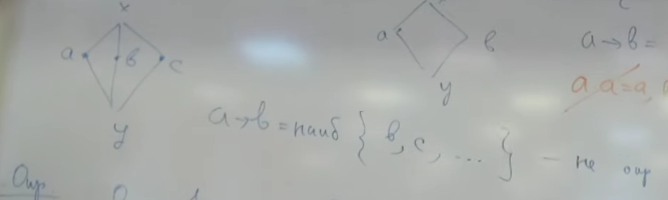
\includegraphics[scale=0.8]{parts/topology_diomant}
    \end{center}
\end{definition}

\begin{definition}
    Решетка с псевдодополнением для всех элементов называется импликативной.
\end{definition}

\begin{definition}[0 и 1] .
    \begin{itemize}
        \item $0$ --- элемент, что $0 \leqslant x $ при всех $x$.
        \item $1$ --- элемент, что $x \leqslant 1 $ при всех $x$.
    \end{itemize}
\end{definition}

\begin{theorem}
    [В импликативной решетке 1 есть всегда] $X, \leqslant$ --- импликативная решетка.
    
    Рассмотрим $a \to a= \text{наиб} \{ c ~|~ q \cdot c \leqslant a\} = \text{наиб} X = 1$.
\end{theorem}

\begin{theorem}
    Рассмотрим $\langle X, \Omega \rangle$ --- импликативная решетка с $0$. Рассмотрим И.И.В.


    Определим оценки $\mathbb{V}  = X$:
    \begin{itemize}
        \item     $\llbracket \alpha \& \beta \rrbracket = \llbracket\alpha \rrbracket \cdot \llbracket\beta \rrbracket$.
        \item     $\llbracket \alpha \vee \beta \rrbracket = \llbracket\alpha \rrbracket + \llbracket\beta \rrbracket$.
        \item     $\llbracket \alpha \to \beta \rrbracket = \llbracket\alpha \rrbracket \to \llbracket\beta \rrbracket$.
        \item     $\llbracket \neg \alpha \rrbracket = \llbracket\alpha \rrbracket \to 0$.
    \end{itemize}

    $\alpha$ истинно, если $\llbracket \alpha \rrbracket = 1$.

    Полученная модель --- корректная модель И.И.В.
\end{theorem}

У нас будет натуральный вывод, интуиция и все такое.

$\overline{\Gamma, \varphi \vdash \varphi}$ (аксиома).

Вывод утверждения в доказательстве $\Gamma \vdash \varphi$.

\[
    \dfrac{\Gamma, \varphi \vdash \psi}{\Gamma \vdash \varphi \to \psi},~~~
    \dfrac{\Gamma, \varphi \vdash \psi~~~ \Gamma \vdash \varphi}{\Gamma \vdash \psi},~~~
    \dfrac{\Gamma, \varphi ~~~ \Gamma \vdash \psi}{\Gamma \vdash \varphi \& \psi},~~~
    \dfrac{\Gamma, \vdash \varphi \& \psi}{\Gamma \vdash \varphi},~~~
    \dfrac{\Gamma, \vdash \varphi \& \psi}{\Gamma \vdash \psi},
\]\[
    \dfrac{\Gamma \vdash \varphi}{\Gamma\vdash\varphi \vee \psi},~~~
    \dfrac{\Gamma \vdash \psi}{\Gamma\vdash\varphi \vee \psi},~~~
    \dfrac{\Gamma, \varphi \vdash \rho~~~ \Gamma, \psi \vdash \rho~~~ \Gamma \vdash \varphi \vee \psi}{\Gamma\vdash\rho},~~~
    \dfrac{\Gamma \vdash \bot }{\Gamma\vdash\varphi}.
\]

В теореме выше нужно добавить, что $\llbracket\bot \rrbracket = 0$.

$\neg \alpha \equiv \alpha \to \bot$.

\endinput
\begin{definition}
    Алгебра Гейтинга~--- импликативная решетка с 0.

    Введем операцию $\sim a \equiv a \to 0$~--- дополнение до 0.
\end{definition}

\begin{definition}
    Булева алегбра~--- Алгебра Гейтинга, где $a + \sim a = 1$.
\end{definition}

\begin{example}
    Булева Алгебра

    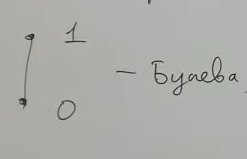
\includegraphics[scale=0.8]{img/bool_algebra}
    
    \begin{itemize}
        \item $\cdot$ соответствует $\&$,
        \item $+$ соответствует $\vee$,
        \item $\to$ соответствует $\to$,
        \item $\sim$ соответствует $\neg$.
    \end{itemize}
\end{example}

Далее $\alpha, \beta$~--- выссказывания в ИИВ.

\begin{definition}
    $\alpha \leqslant \beta$, если $\alpha \vdash \beta$
\end{definition}

\begin{definition}
    $\alpha \approx \beta$, если $\alpha \leqslant \beta$ и $\beta \leqslant \alpha$
\end{definition}

\begin{definition}
    Пусть $\xi$~--- множество всех высказываний ИИВ.
    
    Тогда $[ \xi ]$~--- называется алгеброй Линденбаума $\mathcal{L}$.
\end{definition}

\begin{theorem}
    $\mathcal{L}$ --- Алгебра Гейтинга.
\end{theorem}

\begin{lemma}
    $\mathds{1} = [A \to A]$
\end{lemma}

\begin{proof}
    $\alpha \vdash A \to A$, верно (очевидно), то есть $[\alpha] \leqslant [A \to A]$, то есть $[A \to A] = 1$.
\end{proof}

\begin{theorem}
    $\mathcal{L}$~--- корректная модель ИИВ.
\end{theorem}

\begin{theorem}
    $\mathcal{L}$~--- полная модель ИИВ.

\end{theorem}

\begin{theorem}
    $\vDash \alpha$, то есть $[\alpha] = 1$.

    $1 = [A \to A]$, то есть $[\alpha] =1$, то есть $\beta \leqslant [\alpha]$ при всех $\beta$.
    
    Возьмем $\beta = A \to A$, $A \to A \vdash \alpha$, то есть $A \to A$, $(A \to A) \to \alpha$.

\end{theorem}

\begin{theorem}
    Алгебра Гейтинга --- полная и корректная модель ИИВ.
\end{theorem}

\begin{definition}
    Исчисление дизъюнктно, если для любых $\alpha, \beta\quad \vdash \alpha \lor \beta$ влечёт $\vdash \alpha$ или $\vdash \beta$.
\end{definition}

\begin{theorem}
    ИИВ дизъюнктно.
\end{theorem}

\begin{definition}
    Пусть существует $f: A \to B, \quad A, B$ -- алгебры Гейтинга.    

    $f$ -- гомоморфизм, если $f(0_A) = 0_B\quad f(1_A) = 1_B$ и $f(\alpha \star_A \beta) = f(\alpha) \star_B f(\beta)$
\end{definition}

\begin{definition}   [Геделева Алгебра]
    Это такая алгебра, где $a + b = 1$ влечет $a = 1$ или $b = 1$.
\end{definition}

\begin{definition}
    [$\Gamma (A)$]    
    Пусть $A$~--- алгебра Гейтинга.

    Определим $\gamma: A \to \Gamma(A)$ так:
    $\gamma(x) = \begin{cases}
        \omega, &x = 1_A\\
        x, & x < 1_A\\
    \end{cases}$
    и добавим $1_{\Gamma(A)}$: $t \leqslant 1_\Gamma(A)$, если $t \in \Gamma(A)$.    

    \begin{center}
        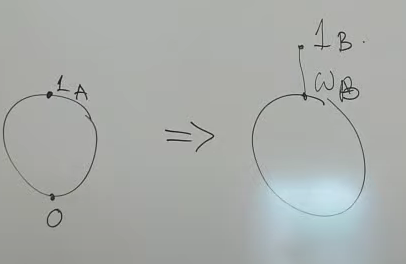
\includegraphics[scale=0.5]{img/gedelerisation.png}    
    \end{center}
\end{definition}

\begin{remark}
    $\Gamma (A)$ неофициально называется Геделеризацией.
\end{remark}

\begin{theorem}
  $\Gamma(A)$ -- Гёделева алгебра.  
\end{theorem}
\begin{proof}
    Пусть $a+b = 1_{\Gamma(A)}$, посмотрим на картинку.
\end{proof}

\begin{statement}
    $\Gamma(\mathcal L)$~--- Гёделева алгебра.
\end{statement}
\begin{proof}
    Определим каноническое отображение $g(x): \Gamma(\mathcal L) \to \mathcal L$\\ 
    $g(x) = \begin{cases}
        1&, x = 1 \text{ или } \omega\\
        x&, \text{ иначе}\\
    \end{cases} $
    \begin{statement}
        $g(x)$ -- гомоморфизм
    \end{statement}
    
\end{proof}

\begin{theorem}
    Рассмотрим ИИВ и алгебры Гейтинга $\mathcal L, \Gamma (\mathcal{L})$
\end{theorem}

\begin{statement}
    Если $g: A \to B$ и $\llbracket\alpha\rrbracket_A = 1_A$, то
    $\llbracket \alpha \rrbracket_B = g(1_A)$.
\end{statement}


\begin{proof}[Доказательство теоремы]

    Рассмотрим $\vdash \alpha \vee \beta$.

    $\Gamma (\mathcal L)$~--- Геделва алгеба, то есть алгебра Гейтинга.
    
    $\llbracket \alpha \lor \beta \rrbracket_{\Gamma(\mathcal L)} = 1_{\Gamma(\mathcal L)}$, 
    т.е. либо $\llbracket \alpha \rrbracket =1_\gamma{\mathcal L}$ либо $\llbracket \beta \rrbracket _{\Gamma(\mathcal L)} = 1_{\Gamma(\mathcal L)}$

    Рассмотрим $g : \Gamma(\mathcal{L}) \to \mathcal{L}$

    $\llbracket \alpha \rrbracket _{\Gamma(\mathcal L )} = 1_{\Gamma(\mathcal L)}$, тогда $\llbracket \alpha \rrbracket _{\mathcal L} = g(1_{\Gamma(\mathcal L)}) = 1_{\mathcal L}$

    т.е. $\vdash \alpha$.
\end{proof}

\begin{definition}
    Модель ИИВ называется табличной, если\begin{itemize}
        \item $\mathbb{V} = \mathcal{S}$;
        \item $\llbracket \alpha \star \beta \rrbracket = f_\star \left( \llbracket \alpha \rrbracket, \llbracket \alpha, \beta \rrbracket \right)$,
        \item  Существует $\true \in \mathcal{S}$ -- выделенная истина $\llbracket \alpha \rrbracket = \true$ тогда и только тогда, когда $\vDash \alpha$
    \end{itemize}
\end{definition}
    \begin{definition}[Модель Крипки]
        Некоторые факты, появившиеся на оси времени в истинном или ложном виде и больше не меняется
        
        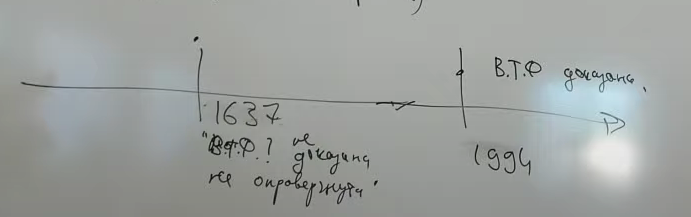
\includegraphics[scale=0.7]{img/kripke_model_greate_ferma_theorem}
    \end{definition}
    
    \begin{note}
        $W$ -- частично упорядоченное множество миров.
    \end{note}

    \begin{definition}
        $\Vdash$

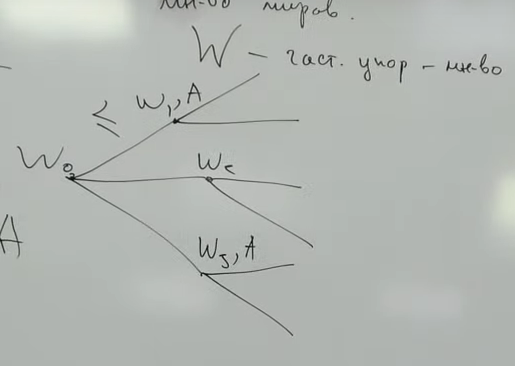
\includegraphics[]{img/forced_variable_worlds}

        \begin{enumerate}
            \item Вынужденность переменной A определяется моделью. При этом, если $W_x \leqslant W_y$, $ W_x\Vdash A$, то $W_y \vDash A$. 
            \item Доопределим $\Vdash$ на все выражения:
            \begin{enumerate}
                \item $W \Vdash A\land B$, если $W \Vdash A$ и $W \Vdash B$
                \item $W \Vdash A\lor B$, если $W \Vdash A$ или $W \Vdash B$
                \item $W \Vdash \neg A$, если нет $W \leqslant W_x$, что $W \Vdash A$
                \item $W \Vdash A \to B$, если во всех $W \leqslant W_x $ из $W_x \Vdash A$ следует $W_x \Vdash B$
            \end{enumerate}
        \end{enumerate}
    \end{definition}

    \begin{theorem}
        У ИИВ нет полной конечной табличной модели.
    \end{theorem}
    \begin{proof}
        $\varphi(u)\bigvee\limits_{i\neq j}^n A_i \to A_{j}$ 

        Пусть $T$~--- модель, $|\mathbb{V}| = n$.

        Рассмотрим $\varphi(n+1)$.  По принципу Дирихле. Есть $A_j$ и $A_i$: $\llbracket A_j \rrbracket = \llbracket A_i \rrbracket$.

        Несложно показать $\llbracket A_i \to A_j = \true$. $\llbracket \varphi(n + 1) \rrbracket = \true$. 
    \end{proof}

\begin{theorem}
    Модель Крипке~--- корректная модель ИИВ.
\end{theorem}

\subsection{Изоморфизм Кари--Ховарда}

\begin{statement}
    $\tau, \sigma$~-- типы. 
    
    $\tau \to \sigma$
    \begin{lstlisting}[mathescape=true]
    f(x : $\tau$): $\sigma$ {
        return g(x);
    }\end{lstlisting}

    $\tau \& \sigma$
    \begin{lstlisting}[mathescape=true]
    f(x: $\tau$, y: $\sigma$)\end{lstlisting}

    $\tau \vee \sigma$
    \begin{lstlisting}[mathescape=true]
    f(x: std:variant<$\tau$, $\sigma$>)\end{lstlisting}

\end{statement}

\begin{definition}
    [Изоморфизм Кари--Ховарда]

    Программа соответствует доказательству. Тип соответствует утверждению. ...

    (всё в интуиционисткой логике)
\end{definition}

\begin{note}
    $f: \neg\neg \alpha \to \alpha $ -- потом подумаем как это интерпретировать.
\end{note}

\endinput

\end{document}